\subsection{\spatialAcronym\ trial subspaces: direct solution approach}\label{sec:direct} 

Direct approaches solve optimization problem~\eqref{eq:tclsrm} by
``transcribing" the infinite-dimensional optimization problem into a finite-dimensional one by discretizing the state and objective functional in time.
The minimization problem is then reformulated as a (non)linear 
optimization problem. A variety of direct solution approaches exist, 
including collocation approaches, spectral  methods, and genetic algorithms.  
In the context of \spatialAcronym\ trial subspaces, the most straightforward direct solution approach consists of the 
following steps: (1) numerically discretize the FOM ODE (and hence the
\textit{integrand} of the objective function in problem~\eqref{eq:obj_gen_slab}) and 
(2) select a numerical quadrature rule to evaluate the \textit{integral}
defining the objective function in~\eqref{eq:obj_gen_slab}.
To this end, we define time grids
$\{\timeWindowArg{n}{i}\}_{i=0}^{\nstepsArg{n}}\subset[\timeStartArg{n},\timeEndArg{n}]$,
$n=1,\ldots,\nslabs$ that
satisfy 
$\timeStartArg{n}=\timeWindowArg{n}{0} \le \cdots \le \timeWindowArg{n}{\nstepsArg{n}} 
 = \timeEndArg{n}$. %\KTC{use cdots, not
%hdots or ldots. Don't use $\defeq$ for the first and last times; these are
%just equalities, i.e., you happen to set them equal to those values, but they
%aren't identically the same:}
Figure~\ref{fig:slab_fig2} depicts such a discretization.
For the purposes of indexing between different windows, we additionally define a function:
$$\indexMapper: (n,i) \mapsto 
\begin{cases}
	(n,i) & n = 1, \; i = 0, \\
	(n,i) & n \geq 1, \; i > 0, \\
\indexMapper(n-1,\nstepsArg{n-1}+i) & n > 1, \; i \le 0.
\end{cases}$$
We now outline the direct solution approach for linear-multistep schemes; the formulation for
other time-integration methods (e.g., Runge--Kutta) follows closely. 
\begin{figure} 
\begin{centering} 
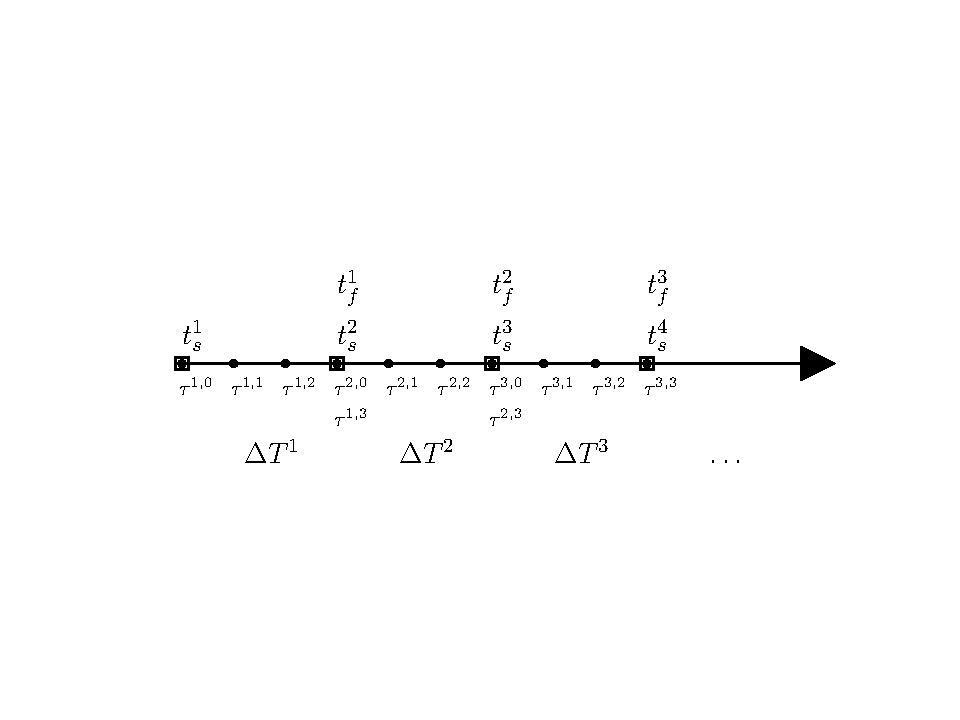
\includegraphics[trim={0.0cm 4.5cm 0cm 3cm},clip,width=1.0\textwidth]{figs/time_grid_timesteps.pdf} 
	\caption{Depiction of the $\nstepsArg{n}+1$ time instances over each window. In the figure, $\nstepsArg{n} = 2$ for all $n$.} 
\label{fig:slab_fig2} 
\end{centering} 
\end{figure}
%We now outline several commonly employed temporal discretization 
%schemes, specifically linear multistep and collocation (Runge--Kutta) methods, that leverage this time-grid to discretize the FOM ODE and 
%objective functional.  

%\subsubsection{Temporal Discretization of the FOM ODE}
%To develop the direct solution approach, we first outline several 
%commonly employed methods used to discretize the FOM ODE, and then 
%subsequently demonstrate how these techniques can be used to discretize 
%and solve Eq.~\ref{eq:obj_gen_slab}. To develop the direct solution approach, 
%we start by dividing each time slab $[\timeStartArg{n},\timeEndArg{n}]$ into
%$\nstepsArg{n}$ strictly increasing time-step instances described by,
%$\{\timeWindowArg{n}{i}\}_{i=0}^{\nstepsArg{n}}$, with  \begin{align*}
%&\timeWindowArg{n}{0} \le \ldots \le \timeWindowArg{n}{\nstepsArg{n}} , \\
%&\timeWindowArg{n}{0} \defeq \timeStartArg{n}, \\
%&\timeWindowArg{n}{\nstepsArg{n}} \defeq \timeEndArg{n}. 
%%\timeWindowArg{n}{0} = \timeStartArg{n}, \timeWindowArg{n}{\nstepsArg{n}} =
%%\timeEndArg{n}
%\end{align*}
\subsubsection{Linear multistep schemes}\label{sec:lmm}
Linear multistep schemes approximate the solution at time instance $\timeWindowArg{n}{i}$ using the previous $\lmsWidthArg{n}{i}$ time instances, where $\lmsWidthArg{n}{i}$ denotes the number of time steps employed by the scheme at the $i$th time instance of the $n$th window. 
%Discretizing the FOM ODE~\eqref{eq:FOM} with a linear $k$-step scheme at the $i$th time-instance over the $n$th time slab yields,
%\begin{equation}\label{eq:kstep}
%\sum_{j=0}^{\lmsWidthArg{n}{i}} \alpha_j \stateFOMDiscreteArg{n,i-j} = \Delta t^{n,i} \sum_{j=0}^{\lmsWidthArg{n}{i}} \beta_j \velocity(\stateFOMDiscreteArg{n,i-j}),
%\end{equation}
Employing such a method to discretize the FOM ODE yields the sequence of FOM
O$\Delta$Es defined over the $n$th time window
%\footnote{
%To maintain notational simplicity in this section, and handle the case where the linear multistep method employs time instances from the previous window(s), for superscripts $n=1,\ldots,\nslabs$ and $i<0$, we set the superscripts to be $n =n-1, i = \nstepsArg{n-1}+i$ 
%% $\stateFOMDiscreteLMSArg{n}{i} = \stateFOMDiscreteLMSArg{n-1}{\nstepsArg{n-1}+i}$, along with $\timeWindowArg{n}{i} = \timeWindowArg{n-1}{\nstepsArg{n-1}+i}$.
%}, 
\begin{align*}
&\residLMSWArg{n}{i} (\stateFOMDiscreteArg{n,i};\stateFOMDiscreteLMSArg{n}{i-1},\ldots,\stateFOMDiscreteLMSArg{n}{i-\lmsWidthArg{n}{i}}) = \bz, \qquad i=1,\ldots,\nstepsArg{n}
%\begin{cases}
%\stateFOMDiscreteLMSArg{n-1}{0} & n = 2,\ldots,\nslabs \\
%\stateFOMIC & n=1, \end{cases}
\end{align*}
along with the initial condition $\stateFOMDiscreteArg{1,0} = \stateFOMIC$.
Here, $\stateFOMDiscreteArg{n,i} (\approx
\stateFOMArg{}{\timeWindowArg{n}{i}})
\in \RR{\fomdim}$ and $\residLMSWArg{n}{i}$ denotes the FOM O$\Delta$E
residual over the $i$th time instance of the $n$th window  
defined as
\begin{align*}
\residLMSWArg{n}{i} &: (\stateyDiscreteArgnt{i};\stateyDiscreteArgnt{i-1},\ldots,\stateyDiscreteArgnt{i-\lmsWidthArg{n}{i}}) \mapsto  \frac{1}{\Delta t^{n,i}} \sum_{j=0}^{\lmsWidthArg{n}{i}} \alpha^{n,i}_j \stateyDiscreteArgnt{i-j} -  \sum_{j=0}^{\lmsWidthArg{n}{i}} \beta^{n,i}_j \velocity(\stateyDiscreteArgnt{i-j},\timeWindow^{\indexMapper(n,i-j)}), \\
               &: \RR{\fomdim} \otimes \RR{\lmsWidthArg{n}{i}+1} \rightarrow \RR{\fomdim}. 
\end{align*}
Here, $\Delta t^{n,i} \defeq \timeWindowArg{n}{i} - \timeWindowArg{n}{i-1}$
denotes the time step, and
$\alpha^{n,i}_j,\beta^{n,i}_j\in\RR{}$ denote coefficients that 
define the specific type of multistep scheme at the $i$th time instance of the $n$th window. 
%\begin{remark}\label{remark:LMS}
%For notational simplicity, we assume the linear multistep method employs time
%	instances from only within the current time window. In general, the linear
%	multistep method at the $n$th window could be designed to employ multiple
%	time instances from previous time windows. \KTC{What are the implications of
%	this? I suggest removing this and adding a simple condition, maybe with a
%	footnote.}
%\end{remark}
%Employing a linear multistep method for temporal discretization of the FOM ODE leads to the FOM O$\Delta$E over the $n$th slab,
%\begin{align*}
%&\residLMSArg{n,i} (\stateFOMDiscreteArg{n,i},\ldots,\stateFOMDiscreteArg{n,i-k^n(i)}) = \bz, \qquad i=1,\ldots,\nstepsArg{n}, \\
%&\stateArgnt{n,0} = \begin{cases}
%\stateFOMDiscreteArg{n-1,\nstepsArg{n-1}} & n = 2,\ldots,\nslabs, \\
%\stateFOMIC & n=1, \end{cases}
%\end{align*}
%where $\residLMSArg{n,i}$ is the discrete linear multistep residual over the $i$th time-step instance of the $n$th slab,
%\begin{align*}
%\residArg{n,i} &: (\stateyDiscreteArgnt{n,i},\ldots,\stateyDiscreteArgnt{n,i-k(i)}) \mapsto  \frac{1}{\Delta t^{n,i}} \sum_{j=0}^{\lmsWidthArg{n}{i}} \alpha_j \stateyDiscreteArgnt{n,i-j} -  \sum_{j=0}^{\lmsWidthArg{n}{i}} \beta_j \velocity(\stateyDiscreteArgnt{n,i-j}),
%\\
%               &: \RR{\fomdim} \otimes \RR{k(i)} \rightarrow \RR{\fomdim}. 
%\end{align*} 
Employing a linear multistep method allows the objective \textit{functional}~\eqref{eq:obj} to be replaced with the objective \textit{function}
%In the above, $\objectiveArgLMS{n}$ is the discrete objective function at the $n$th time window and is defined as
\begin{equation*}%\label{eq:obj_lms}
\begin{split} 
\objectiveArgLMS{n}_{\text{D}} &\vcentcolon
	(\stateyDiscreteArgnt{1},\ldots,\stateyDiscreteArgnt{\nstepsArg{n}};
	\stateyDiscreteArgnt{0},\ldots,\stateyDiscreteArgnt{-\lmsWidthArg{n}{1}+1})
	\mapsto 
\frac{1}{2} \sum_{i=1}^{\nstepsArg{n}} \quadWeightsLMSScalarArg{n}{i} [\residLMSWArg{n}{i}(\stateyDiscreteArgnt{i};\stateyDiscreteArgnt{i-1},\ldots, \stateyDiscreteArgnt{i-\lmsWidthArg{n}{i})})]^T  \stweightingMatArgt{n}{\timeWindowArg{n}{i}} \residLMSWArg{n}{i}(\stateyDiscreteArgnt{i};\stateyDiscreteArgnt{i-1},\ldots, \stateyDiscreteArgnt{i-\lmsWidthArg{n}{i}}), \\
&\vcentcolon \RR{\fomdim} \otimes \RR{\nstepsArg{n} + \lmsWidthArg{n}{1}} \rightarrow
\RR{}_+, 
\end{split}
\end{equation*}
where $\quadWeightsLMSScalarArg{n}{i} \in \RRplus$ are quadrature weights.  

\methodAcronym\ with the direct approach and a linear multistep method sequentially computes the solutions
$\approxstateDiscreteArg{n,1},\ldots,\approxstateDiscreteArg{n,\nstepsArg{n}}$,
$n=1,\ldots,\nslabs$, that satisfy
%	\KTC{What is $\genstate^{n-1}(\timeEndArg{n-1} ) $ doing here? Two problems
%	(1) there is no notion of a generalized coordinate $\genstate$ yet, and (2)
%	this should be the discrete solution, not the exact solution evaluated at
%	the final time.} \EP{You are correct, I think there is an error now in the minimize term though. It was $\in \trialspace\otimes \RR{\lmsWidthArg{n}{i}+1}$, it should be $\trialspace\otimes \RR{\nstepsArg{n}+1}$}
\begin{align*}
	&\underset{(\stateyDiscreteArgnt{1},\ldots,\stateyDiscreteArgnt{\nstepsArg{n}}) \in ( \trialspace + \stateInterceptArg{n}) \otimes \RR{\nstepsArg{n}}}{\text{minimize } }
\objectiveArgLMS{n}_{\text{D-S}} (\stateyDiscreteArgnt{1},\ldots,\stateyDiscreteArgnt{\nstepsArg{n}}), 
%%& \text{subject to} \hspace{0.2 in}  \stateyDiscreteArg{0} =
%%\begin{cases} \basisspaceArg{n} \spatialICDiscrete + \stateInterceptArg{n}& n = 2,\ldots,\nslabs,\\
%\basisspaceArg{1} \genstateICOne  + \stateInterceptArg{1}& n=1. \end{cases} 
\end{align*}
where
\begin{equation*}
\begin{split}
\objectiveArgLMS{n}_{\text{D-S}} &\vcentcolon  (\stateyDiscreteArgnt{1},\ldots,\stateyDiscreteArgnt{\nstepsArg{n}}) \mapsto \objectiveArgLMS{n}(\stateyDiscreteArgnt{1},\ldots,\stateyDiscreteArgnt{\nstepsArg{n}}; \approxstateDiscreteArg{\indexMapper(n,0)},\ldots,\approxstateDiscreteArg{\indexMapper(n,-\lmsWidthArg{n}{1}+1)}), \\
&\vcentcolon \RR{\fomdim} \otimes \RR{\nstepsArg{n}} \rightarrow \RR{}_+,
\end{split}
\end{equation*}
with the initial condition $\approxstateDiscreteArg{1,0} = \basisspaceArg{n}\basisspaceTArg{n} (\stateFOMIC - \stateInterceptArg{n}) + \stateInterceptArg{n}$.
%We additionally set $\approxstateDiscreteArg{1,0} = \projectorSpatialArg{n}(\stateFOMIC)$, where
%$\projectorSpatialArg{n} : \RR{\fomdim} \rightarrow \trialspaceArg{n}$ is the $\elltwo$-orthogonal projector 
%$$\projectorSpatialArg{n} : \stateyDiscreteArgnt{} \mapsto  \basisspaceArg{n}\basisspaceTArg{n} (\stateyDiscreteArgnt{} - \stateInterceptArg{n}) + \stateInterceptArg{n} .$$

%where 
%\begin{align*}
%\residArg{n,i} &: (\stateyArgnt{n,i},\ldots,\stateyArgnt{n,i-k(i)}) \mapsto  \sum_{j=0}^k \alpha_j \stateyArgnt{n,i-j} = \Delta t^{n,i} \sum_{j=0}^k \beta_j \velocity(\stateyArgnt{n,i-j}),
%\\
%               &: \RR{\fomdim} \otimes \RR{k(i)} \rightarrow \RR{\fomdim}, 
%\end{align*} 
%is the discrete residual resulting from the linear multistep scheme and 
%\methodAcronym\ solves the minimization problem over each time window, 
%\begin{align*}
%&\approxstateDiscreteArg{n,0},\ldots,\approxstateDiscreteArg{n,\nstepsArg{n}} = \underset{\stateyDiscreteArgnt{n,0},\ldots,\stateyDiscreteArgnt{n,\nstepsArg{n}} \in \trialspace}{\text{arg\,min } }
%\objectiveArgLMS{n} (\stateyDiscreteArgnt{n,0},\ldots,\stateyDiscreteArgnt{n,\nstepsArg{n}}) \\
%& \text{subject to} \hspace{0.2 in}  \approxstateDiscreteArg{n,0} =
%\begin{cases} \approxstateDiscreteArg{n-1,\nstepsArg{n-1}} & n = 2,\ldots,\nslabs,\\
%\approxstateIC & n=1. \end{cases} \end{align*}

Equivalently, \methodAcronym\ with the direct approach and a linear multistep method sequentially computes the generalized
	coordinates
	$\genstateDiscreteArg{n,1},\ldots,\genstateDiscreteArg{n,\nstepsArg{n}}$,
	$n=1,\ldots,\nslabs$ 
with $\genstateDiscreteArg{n,i}(\approx
	\genstateArgnt{n}(\timeWindowArg{n}{i}))\in\RR{\romdimArg{n}}$
	that satisfy
\begin{equation}\label{eq:obj_gen_lms_final}
\begin{split}
	&
	\underset{(\genstateyDiscreteArg{1},\ldots,\genstateyDiscreteArg{\nstepsArg{n}})\in\RR{\romdimArg{n}}\otimes \RR{\nstepsArg{n}}}{\text{minimize } }
\objectiveArgLMS{n}_{\text{D-S}} (\basisspaceArg{n} \genstateyDiscreteArg{1} + \stateInterceptArg{n},\ldots,\basisspaceArg{n} \genstateyDiscreteArg{\nstepsArg{n}} + \stateInterceptArg{n}). 
%& \text{subject to} \hspace{0.2 in}
%\genstateyDiscreteArg{0} =
%\begin{cases} \genspatialICDiscrete  & n = 2,\ldots,\nslabs \\
%\genstateICOne& n=1. \end{cases} 
\end{split}
\end{equation}
%\begin{equation}\label{eq:obj_gen_lms_final}
%\begin{split}
%& \genstateDiscreteArg{n,0},\ldots,\genstateDiscreteArg{n,\nstepsArg{n}}  = \underset{\genstateyDiscreteArg{n,0},\ldots,\genstateyDiscreteArg{n,\nstepsArg{n}}}{\text{arg\,min } }
%\objectiveArgLMS{n} (\basisspace \genstateyDiscreteArg{n,0} + \stateIntercept,\ldots,\basisspace \genstateyDiscreteArg{n,\nstepsArg{n}} + \stateIntercept) \\ 
%& \text{subject to} \hspace{0.2 in}
%\genstateDiscreteArg{n,0} =
%\begin{cases} \genstateDiscreteArg{n-1, \nstepsArg{n-1}} & n = 2,\ldots,\nslabs \\
%\basisspace^T(\stateFOMIC - \stateIntercept)& n=1. \end{cases} 
%\end{split}
%\end{equation}
The optimization problem takes the form of a \textit{weighted least-squares
	problem}. 
We emphasize that optimization problem~\eqref{eq:obj_gen_lms_final} associates
	with an \spatialAcronym\ trial subspace characterized by a reduction in
	spatial complexity, but no reduction in temporal complexity.
 
The minimization problem~\eqref{eq:obj_gen_lms_final} requires specification of the quadrature weights (and hence the integration scheme used to discretize 
the objective functional). Typically, the same integration scheme used to discretize the FOM ODE is employed for consistency~\cite{colloc_review}; e.g., if a  
backward Euler method is used to discretize the FOM ODE, then a backward Euler method is the used to numerically integrate the objective functional.

\begin{remark}
For the limiting case where $\nstepsArg{n} = 1$, $n=1,\ldots,\nslabs$ such that the window size is equivalent to the time step (i.e., $\DeltaSlabArg{n} = \timeWindowArg{n}{1} - \timeWindowArg{n}{0}$), uniform 
quadrature weights are used, a uniform trial space is employed (i.e., $\trialspaceArg{n} = \trialspace$ and $\stateInterceptArg{n} = \stateInterceptArg{}, n=1,\ldots,\nslabs$), the weighting matrices are taken to be
$\stweightingMatOneArg{n} = \lspgWeightingArg{}, n=1,\ldots,\nslabs$, and the
	time instances correspond to the time grid used for time discretization $\timeWindowArg{n}{1} = t^n$, $n=1,\ldots,\nslabs$, then 
$\approxstateDiscreteArg{n,1}  = \approxstateLSPG^n$, $n=1,\ldots,\nslabs$ and  
\methodAcronym\ with \spatialAcronym\ trial
	subspaces solved via the direct approach recovers the LSPG approach. 
\end{remark} 
\subsubsection{Solution to the least-squares problem through the Gauss--Newton
	method}
	Problem \eqref{eq:obj_gen_lms_final} corresponds to a discrete least-squares
	problem, which is nonlinear if the full-order-model velocity $\velocity$ is nonlinear in
	its first argument. 
A variety of algorithms exist for solving nonlinear least-squares problems,
	including the Gauss--Newton method, and the Levenberg--Marquardt method.
 The numerical experiments
	presented in this work consider nonlinear dynamical systems and are solved
	via the Gauss--Newton method; as such, we outline this approach here. 

Defining a ``vectorization" function 
\begin{align*}
 \unroll &\vcentcolon (\stateyDiscreteArg{1},\ldots,\stateyDiscreteArg{m} ) \mapsto \begin{bmatrix} [\stateyDiscreteArg{1}]^T & \ldots & [\stateyDiscreteArg{m}]^T \end{bmatrix}^T  \\
&\vcentcolon \RR{p} \otimes \RR{m} \rightarrow \RR{pm},
\end{align*}
the vectorized generalized coordinates over the $n$th time window are 
defined as 
\begin{equation*}
\genstatecollocMatSlabArg{n} \defeq 
\unroll (\genstateDiscreteArg{n,1},\ldots,\genstateDiscreteArg{n,\nstepsArg{n}} ).
\end{equation*}
We now define the weighted space--time residual over the entire window as
\begin{equation*}
\residLMSSlabArg{n} : \genstatecollocMatySlabArg{} \mapsto \begin{bmatrix}
 \sqrt{\frac{\quadWeightsLMSScalarArg{n}{1}}{2}} \stweightingMatOneArg{n} \residLMSArg{n,1}( \basisspaceArg{n} \genstateyDiscreteArgnt{1} + \stateInterceptArg{n}; 
%\residLMSArg{n,0}( \basisspaceArg{n} \genstateyDiscreteArgnt{0} + \stateInterceptArg{n}),
 \approxstateDiscreteArg{\indexMapper(n,0)},
\ldots , \approxstateDiscreteArg{\indexMapper(n,1 - \lmsWidthArg{n}{1}) }   ) \\
\vdots \\
 \sqrt{\frac{\quadWeightsLMSScalarArg{n}{\nstepsArg{n}}}{2}} \stweightingMatOneArg{n} \residLMSArg{n,\nstepsArg{n}}( \basisspaceArg{n} \genstateyDiscreteArgnt{\nstepsArg{n}} + \stateInterceptArg{n}; \basisspaceArg{n} \genstateyDiscreteArgnt{\nstepsArg{n}-1} + \stateInterceptArg{n} ,  \ldots, \basisspaceArg{n} \genstateyDiscreteArgnt{\nstepsArg{n} - \lmsWidthArg{n}{\nstepsArg{n}} } + \stateInterceptArg{n} ) \\
\end{bmatrix},
\end{equation*}
where $\genstatecollocMatySlabArg{} \equiv \unroll (\genstateyDiscreteArg{1},\ldots,\genstateyDiscreteArg{\nstepsArg{n}} )$ and, for $i \le 0$,
\begin{equation}\label{eq:wls_genspatial_direct_args}
\genstateyDiscreteArgnt{n,i}  \equiv 
\begin{cases}
\genstateDiscreteArg{\indexMapper(n,i)}  & n = 2,\ldots,\nslabs,  \\
\genstateICOne  & n = 1. 
\end{cases}
\end{equation}
We note that
\begin{equation*}
\objectiveArgLMS{n}_{\text{D-S}} \bigg( \basisspaceArg{n} \genstateDiscreteArg{n,1} + \stateInterceptArg{n},\ldots,\basisspaceArg{n} \genstateDiscreteArg{n,\nstepsArg{n}} + \stateInterceptArg{n} \ \bigg) 
=
\bigg[\residLMSSlabArg{n}  (\genstatecollocMatSlabArg{n}) \bigg]^T \bigg[ \residLMSSlabArg{n}(\genstatecollocMatSlabArg{n}) \bigg].
\end{equation*} 
Using these definitions, Algorithm~\ref{alg:colloc_gn} presents the standard
Gauss--Newton method. Each Gauss--Newton iteration consists of three fundamental steps: (1)
compute the FOM O$\Delta$E residual given the current guess, (2) compute the
Jacobian of the residual over the time window, and (3) solve the linear least-squares problem and update the guess. 

The practical implementation of the Gauss--Newton algorithm requires an
efficient method for computing the Jacobian of the residual over the time
window
${\partial \residLMSSlabArg{n}}/{\partial \genstatecollocMatySlabArg{}}$.
For this purpose, we can leverage the fact that this Jacobian is a block lower
triangular matrix with the following sparsity pattern (for $\lmsWidthArg{n}{i} = 1$,
$i=1,\ldots,\nstepsArg{n}$): 
\begin{equation*} \begin{bmatrix*}[l]
\matshapea & \\%[-5pt]
 \matshapea & \matshapea & \\%[-5pt]
 & \matshapea  & \matshapea & \\%[-5pt]
&  & \ddots & \\%[-5pt]
 & &  & \matshapea &  \matshapea 
\end{bmatrix*},
% \begin{bmatrix*}[c]
%\matshapeb & \\[-5pt]
% & \hspace{-12pt}\matshapea & \\[-5pt]
% &  & \hspace{-12pt}\matshapea & \\[-5pt]
%&  & \hspace{5pt} \ddots & \\[-5pt]
% & &  & & \hspace{-15 pt} \matshapea 
%\end{bmatrix*}.
\end{equation*}
where each block comprises an $\fomdim \times \romdimArg{n}$ dense matrix.
In particular, solution techniques can leverage this structure, e.g., to
efficiently compute Jacobian--vector products.
Another consequence of this sparsity pattern is that the normal equations
arising at each Gauss--Newton iteration 
comprise a banded block system that can also be exploited.

\begin{remark}\label{remark:gaussnewton}\textit{(Acceleration of the
	Gauss--Newton Method)}\\
	The principal cost of a Gauss--Newton method is often the formation of the Jacobian matrix. A variety of techniques aimed at 
reducing this computational burden exist; Jacobian-free Newton--Krylov
	methods~\cite{jfnk}, Broyden's method~\cite{broyden} (as explored in
	Ref.~\cite{carlberg_thesis}, Appendix A), and frozen Jacobian approximations
	are several such examples. Further, the space--time formulation introduces
	an extra dimension for parallelization that can be exploited to furture
	reduce the wall time. The investigation of these additional, potentially
	more efficient, solution algorithms is a topic of future work. 
\end{remark}
%\subsubsection{Jacobian-Free Implementation}
%The dominant cost of the Gauss Newton algorithm is the computatation of the action of the Jacobian matrix on the trial basis. To alleviate this burden, the following Jacobian-free method is proposed:
\begin{algorithm}
\caption{\spatialAcronym\ trial subspace: algorithm for the direct solution technique with the Gauss--Newton method and a linear multistep method over the $n$th window}
\label{alg:colloc_gn}
\SetKwInOut{Input}{Input}\SetKwInOut{Output}{Output}
\Input{tolerance, $\epsilon$; initial guess, $\genstateGuessDiscreteArg{n,1}{0},\ldots,\genstateGuessDiscreteArg{n,\nstepsArg{n}}{0}$}%; initial condition $\genstateDiscreteArg{n,0}$}
\Output{Solution to least squares problem, $\genstatecollocMatSlabArg{n}$} 
\textbf{Online Steps}: \\
$\text{converged} \leftarrow \text{false}$ \Comment{Set convergence checker} \\
$\genstatecollocMatSlabArg{n}_0 \leftarrow \unroll(\genstateGuessDiscreteArg{n,1}{0},\ldots,\genstateGuessDiscreteArg{n,\nstepsArg{n}}{0})$ \Comment{Assemble generalized coordinates over window} \\
$k \leftarrow 0$ \Comment{Set counter}\\
\While{\text{not converged}}
{
%\For{$i=1,\hdots,\nstepsArg{n}$}{
%  \For{$j=1,\hdots,\ncollocArg{n}{i}$}{
%Compute: $\approxstateArgnt{n,i}  =  \basisspace  \genstateDiscreteArg{n,i} + \stateIntercept$ 
%\Comment{Compute state} \\
%Compute: $\velocity(\basisspace \genstateDiscreteArg{n,i} + \stateIntercept ) $ \Comment{Compute velocity at each time-step instance}\\
%Compute: $\residLMSArg{n,i}(\basisspace \genstateDiscreteArg{n,i} + \stateIntercept, \ldots , \basisspace \genstateDiscreteArg{n,i - k^n(i)} + \stateIntercept) $  \Comment{Compute residual} \\
%}
$\mathbf{r} \leftarrow \residLMSSlabArg{n}(\genstatecollocMatSlabArg{n}_k)$ \Comment{Compute weighted residual over window} \\
$\mathbf{J} \leftarrow  
\frac{\partial \residLMSSlabArg{n}}{\partial \genstatecollocMatySlabArg{}}(\genstatecollocMatSlabArg{n}_k) 
$ \Comment{Compute weighted residual-Jacobian over window} \\
%Compute: $[\jacobianSlabArg{n}]^T \jacobianSlabArg{n}$ \Comment{Compute system matrix for the normal equations} \\
%Compute: $[\jacobianSlabArg{n}]^T \residLMSSlabArg{n}(\genstatecollocMatSlabArg{n}_k)$ \Comment{compute RHS for normal equations} \\
\uIf{ $\norm{ \mathbf{J}^T\mathbf{r}  } \le \epsilon$ }{
{\text{converged} $\leftarrow$ \text{true}}  \Comment{Check and set convergence based on gradient norm} \\
Return: $\genstatecollocMatSlabArg{n} = \genstatecollocMatSlabArg{n}_{k+1} $ \Comment{Return converged solution}\\
}
\Else{
 Compute  $\Delta  \genstatecollocMatSlabArg{n} $ that minimizes $\norm{ \mathbf{J} \Delta \genstatecollocMatSlabArg{n} +\mathbf{r}}^2$ \Comment{Solve the linear least-squares problem} \\
% Compute  $\Delta  \genstatecollocMatSlabArg{n} $ satisfying $ [\mathbf{J}]^T \mathbf{J} \Delta \genstatecollocMatSlabArg{n}=  -\mathbf{J}^T\mathbf{r}$ \Comment{Solve the normal equations} \\
$\alpha \leftarrow \text{linesearch}(\Delta  \genstatecollocMatSlabArg{n} ) $ \Comment{Compute $\alpha$ based on a line search, or set to 1.}\\
$\genstatecollocMatSlabArg{n}_{k+1} \leftarrow \genstatecollocMatSlabArg{n}_k + \Delta \genstatecollocMatSlabArg{n}$ \Comment{Update guess to the state} \\
}
$k\leftarrow k+1$
}
\end{algorithm}


%\input{direct_collocation}

\subsection{\spatialAcronym\ trial subspaces: indirect solution approach}\label{sec:indirect}
In contrast to the direct approach,
indirect methods ``indirectly" solve the minimization
problem~\eqref{eq:tclsrm} by solving the Euler--Lagrange
equations~\eqref{eq:lspg_continuous}--\eqref{eq:lspg_adjoint} associated with
stationarity. This
system comprises a coupled two-point boundary value
problem. Several techniques have
been devised to solve such problems, 
including shooting methods, multiple shooting
methods~\cite{multiple_shooting}, and the forward--backward sweep
method~\cite{fbs} (FBSM).  This work explores using the FBSM. 

%Solving this coupled problem is significantly more challenging and
%computationally expensive than the standard Galerkin and LSPG methods as it
%requires converging both the forward and backward solve. It is emphasized,
%however, that the entire forward-backward system is compatable with
%hyper-reduction techniques and thus is entirely independent of the full-order
%model size. In addition, as the approach is minimizing the entire space-time
%residual, we expect it to be capable of providing stable and accurate
%solutions in cases where the standard Galerkin and LSPG methods can not.
%Obtaining numerical solutions to Eq.~\ref{eq:lspg_continuous} requires three
%ingrediants: \begin{enumerate} \item Solution strategy for solving the
%coupled forward and backwards problems \item Time discretization schemes for
%the forward and backward problems \item Efficient strategy for evaluating the
%action of the Jacobian transpose on a vector \end{enumerate}

\subsubsection{Forward--backward sweep method (FBSM)}\label{sec:FBSM}
%\subsubsection{Solution Strategy} Solving Eq.~\ref{eq:lspg_continuous} is
%made challenging by the fact that it is a coupled two-point boundary value
%problem. The forward problem is coupled to the backwards adjoint problem,
%while the backwards adjoint sytem is coupled to the forward problem. The
%problem is thus inherently implicit. The most popular techniques to solve
%these types of two-point boundary value problems are shooting methods,
%multiple shooting methods, fully-implicit methods, and the forward backward
%sweep (FBS) method. This work explores using the FBS method. 

%The most straightforward approach to solving Eq.~\ref{eq:lspg_continuous} is
%to 1.) discretized both the forward and backwards problems in time and 2.)
%form and solve the resulting (implicit) nonlinear space-time system. In
%practice, however, this technique may not be practical for larger
%time-windows due to the size of the resuling nonlinear problem. 

Until convergence, the FBSM alternates between solving the
system~\eqref{eq:lspg_continuous} \textit{forward} in time given a fixed value
of the costate, and solving the adjoint equation~\eqref{eq:lspg_adjoint}
\textit{backward} in time given a fixed value for the generalized coordinates.
Typically, the system~\eqref{eq:lspg_continuous} is solved first given an
initial guess for the costate.
%
%consists of the following steps. First, the
%system~\eqref{eq:lspg_continuous} is (numerically) solved \textit{forward} in
%time using an initial guess of the costate to obtain an initial solution for
%the generalized coordinates. Next, given this initial solution for the
%generalized coordinates, the adjoint equation~\eqref{eq:lspg_adjoint} is
%solved \textit{backward} in time for an updated costate solution.
%approximation to the generalized coordinates. This gives a new estimate to the
%costate, which is then used to again solve the forward problem to obtain
%a new estimate of the generalized coordinates. This process is continued until
%convergence. 
Algorithm~\ref{alg:st_iter} outlines the algorithm, which 
contains three parameters: the relaxation factor $\rho \le 1$, the growth factor
$\fbsmGrowth \ge 1$, and the decay factor $\fbsmDecay \ge 1$. The relaxation factor controls the rate at which the costate seen by~\eqref{eq:lspg_continuous} is updated. The
closer $\rho$ is to unity, the faster the algorithm will converge.
For large window sizes, however, a large a value of $\rho$ can lead to an unstable iterative process. 
In practice, a line search is used to compute an acceptable value for the
relaxation factor $\rho$. The line search presented in Algorithm~\ref{alg:st_iter} adapts the relaxation factor
according to the objective. Convergence properties of the FBSM method are
presented in Ref.~\cite{McAsey2012ConvergenceOT}, which shows that the
algorithm will converge for a sufficiently small 
value of $\rho$.

\begin{algorithm} \caption{\spatialAcronym\ trial subspace: algorithm for the FBSM over the $n$th window.} \label{alg:st_iter} 
\SetKwInOut{Input}{Input}\SetKwInOut{Output}{Output}
\Input{tolerance, $\epsilon$; relaxation factor, $\rho \le 1$; growth factor, $\fbsmGrowth \ge 1$; decay
factor, $\fbsmDecay \ge 1$} 
\Output{Stationary point, $\genstateArgnt{n}$ }
\textbf{Online Steps:}\\ 
$\genstate^n_0 \leftarrow \bz$ \Comment{Set initial guess for state} \\
$\controllerArgnt{n} \leftarrow \boldsymbol 0$ \Comment{Set initial
guess for costate}\\ 
$\text{Compute } \genstateArgnt{n}_1 \text{ satisfying }  \massArg{n} \genstateDotArgnt{n}_1(t)  -  \basisspaceTArg{n} \stweightingMatArg{n}
\velocity(\veloargsromArg{1}) =  \massArg{n} \controllerArg{n}{t}$ 
% Eq.~\ref{eq:lspg_continuous} with $\adjoint^n(t) = \controllerArg{n}{t}$ to
% obtain $\genstate_0^{n}(t)$ 
\Comment{Solve~\eqref{eq:lspg_continuous}}\\ 
%Set: $\genstate^n_1 = \genstate$ \Comment{Set state} \\
%$\objectiveArg{n}({\genstate_1^n(t)})$
%\Comment{Evaluate objective function}\\
$i \leftarrow 1$ \Comment{Set counter}\\
\While{$\epsilon \le \int_{\timeStartArg{n}}^{\timeEndArg{n}} \norm{\genstate^n_{i}(t) - \genstate^n_{i-1}(t) }dt $}{
\small{
\begin{multline*}
\text{ Compute } \adjointArgnt{n} \text{ satisfying }
\massArg{n} \adjointDotArg{n}{t}  + \basisspaceTArg{n} \bigg[\frac{\partial \velocity}{\partial \stateyDiscrete}(\basisspaceArg{n} \genstate^n_i(t) + \stateInterceptArg{n},t) \bigg]^T \stweightingMatArg{n} \basisspaceArg{n} \adjointArg{n}{t}= \\ -\bigg[\basisspaceTArg{n} \bigg[ \frac{\partial \velocity}{\partial \stateyDiscrete} ( \basisspaceArg{n} \genstate^n_i(t) + \stateInterceptArg{n},t) \bigg]^T \stweightingMatArg{n} \bigg( \mathbf{I} -   \basisspaceArg{n} [\massArg{n}]^{-1} \basisspaceTArg{n} \stweightingMatArg{n} \bigg)  \bigg( \basisspaceArg{n} \dot{\genstate}_i^n(t)   -   \velocity( \basisspaceArg{n} \genstate_i^n(t)  +\stateInterceptArg{n},t) \bigg) \bigg] 
\end{multline*} }
\Comment{Solve~\eqref{eq:lspg_adjoint} to obtain guess to costate} \\
%Solve Eq.~\ref{eq:lspg_adjoint} with $\genstate^n(t) = \genstate^n_i(t)$ to obtain $\adjoint^n(t)$ \\
$\controllerArgnt{n}  \leftarrow \rho \controllerArgnt{n} + (1 - \rho) \adjointArgnt{n}$ \Comment{Weighted update to costate}\\
$i \leftarrow i+1$ \Comment{Update counter}\\
$\text{Compute }\genstateArgnt{n}_i \text{ satisfying } \massArg{n} \genstateDotArgnt{n}_i(t)   -  \basisspaceTArg{n} \stweightingMatArg{n} \velocity(\basisspaceArg{n} \genstate^n_i(t) + \stateInterceptArg{n},t) = \massArg{n} \controllerArg{n}{t} $
\Comment{Solve~\eqref{eq:lspg_continuous}}\\
%$\objectiveArg{n}({\genstate_i^n(t)})$ \Comment{Evaluate objective function}\\
\uIf{ $\objectiveArg{n}({\basisspaceArg{n}\genstate_i^n + \stateInterceptArg{n}\otimes \onesFunctionArg{n}}) \le \objectiveArg{n}({\basisspaceArg{n}\genstate_{i-1}^n + \stateInterceptArg{n}\otimes \onesFunctionArg{n}})$}
{
$\rho \leftarrow \text{min}(\rho \fbsmGrowth,1)$ \Comment{Grow the relaxation factor}\\
}
\Else{
$\rho \leftarrow \frac{\rho }{ \fbsmDecay}$ \Comment{Shrink the relaxation factor}\\ 
$\genstate_i^{n} \leftarrow  \genstate_{i-1}^{n}$ \Comment{Reset state to value at previous iteration}
}
}
Return converged solution, $\genstateArgnt{n}= \genstateArgnt{n}_i$
\end{algorithm}
\subsubsection{Considerations for the numerically solving the forward and
backward systems}
The FBSM requires solving the forward~\eqref{eq:lspg_continuous} and
backward~\eqref{eq:lspg_adjoint} systems, both of which are defined at the time-continuous level. 
The numerical implementation of the FBSM requires two main ingredients: (1) temporal discretization schemes for the forward and backward problems and (2) 
an efficient method for computing terms involving the transpose of the
Jacobian of the velocity.

This work employs linear multistep schemes for time discretization of the
forward and backward problems. As described in Section \ref{sec:lmm},
temporal discretization is achieved by introducing $\nstepsArg{n} + 1$ time
instances over each time window.

The second ingredient, namely devising an efficient method for computing terms
involving the transpose of the Jacobain of the velocity,
can be challenging if one
does not have explicit access to this Jacobian or it is too costly to
compute. We discuss two methods that can be used to evaluate such terms
that appear in the forward system~\eqref{eq:lspg_adjoint}:
\begin{enumerate}
\item \textit{Jacobian-free approximation}: A non-intrusive way to evaluate
	these terms is to recognize that all terms including the transpose of the
		Jacobian of the velocity are left multiplied by the transpose of the
		spatial trial basis; this can be manipulated as
$$\basisspaceTArg{n} \bigg[\frac{\partial \velocity}{\partial \stateyDiscrete}
		(\veloargsromn)\bigg]^T = \bigg[  \frac{\partial \velocity}{\partial
		\stateyDiscrete} (\veloargsromn) \basisspaceArg{n} \bigg]^T,$$
		which exposes the ability to approximate rows of this matrix via
		finite differences, e.g., via forward differences as
$$\frac{\partial \velocity}{\partial \stateyDiscrete}(\veloargsromn)
		\basisvec_i^n \approx \frac{1}{\epsilon}\bigg(
		\velocity(\basisspaceArg{n}\genstateArg{n}{t} + \stateInterceptArg{n} +
		\epsilon \basisvec_i^n,t) - \velocity(\veloargsromn) \bigg),\quad
		i=1,\ldots,\romdimArg{n},$$
which requires $\romdimArg{n}+1$ evaluations of the velocity. 

\item \textit{Automatic differentiation}: A more intrusive, but exact
	method for computing these terms is
		through automatic differentiation (AD), which evaluate derivatives of
		functions (e.g., Jacobians, vector-Jacobian products) in a numerically
		exact manner by recursively applying the chain rule. The numerical
		examples presented later in this work leverage AD. The principal drawback
		of this approach is their intrusiveness, which may prevent them from
		practical application, e.g., in legacy codes.
		\KTC{EP: verify this paragraph.}
\end{enumerate}

\KTC{HERE}
\begin{remark}\label{remark:fbsm}(Acceleration of Indirect Methods)
The FBSM is a simple iterative method for solving the coupled two-point boundary value problem. For large time windows, however, the FBSM may require many 
forward--backward iterations for convergence. More sophisticated solution techniques, such as a multiple FBSM method or multiple shooting methods, promise 
to reduce this cost. Analyses of additional solution techniques will be a subject of future work.
\end{remark}

